\Chapter{Projektablauf}

\Section{Aufgabe}

Die Aufgabe bestand darin, einen funktionsf\"ahigen Prozessor auf Basis der RISC-V Instruction Set Architecture zu entwickeln, der auf dem FPGA des gegebenen Entwicklungsboards (\textit{Spartan-3A FPGA Starter Kit}) l\"auft.
\begin{figure}[H]
	\centering
		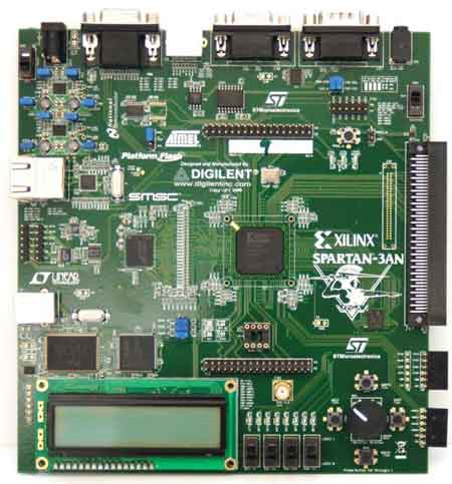
\includegraphics[width=0.3\textwidth]{Board.png}
	\caption{Das verwendete Entwicklungsboard von oben, der FPGA liegt zentral  (ANDERES BILD?)}
	\label{fig:board}
\end{figure}
\Section{Basisziele}


Als Mindestanforderung sollte ein Prozessor mit Kompatibilit\"at zur \textit{RV32I Base Integer Instruction Set} implementiert werden. Ausgenommen davon sind die Befehle FENCE, FENCE.I, SCALL und SBREAK, da keine Hardwareunterst\"utzung f\"ur den Multitaskingbetrieb ben\"otigt wird.

Um die Funktionsf\"ahigkeit des Prozessors auch nach au{\ss}en sichtbar zu machen und keine Black-Box zu erstellen soll die M\"oglichkeit der Interaktion \"uber die Schnittstellen und Pins des Boards bestehen. Insbesondere soll zum Debugging eine grafische Registerausgabe \"uber den VGA-Port an einem Monitor m\"oglich sein.\footnote{Siehe dazu auch Pflichtenheft vom 02.06.16 bzw. 12.11.16}

\Section{Erweiterungsziele}

Aufgrund der Modularit\"at von RISC-V bietet es sich an mindestens eine Erweiterung zu implementieren, n\"amlich die \textit{RV32M Standard Extension for Integer Multiplication and Division}, die Multiplikations- und Divisionsbefehle beinhaltet. Zudem soll die rudiment\"are Ausgabe um einen Textmodus erweitert werden, sodass mittels Memory-Mapping ASCII-Zeichen auf dem Monitor ausgegeben werden k\"onnen. Zum Demonstrieren der Funktionalit\"at soll au{\ss}erdem ein auf dem Prozessor lauff\"ahiges Spiel entwickelt werden. Um auch Daten\"ubertragung mit der Au{\ss}enwelt zu erm\"oglichen soll die serielle Schnittstelle genutzt werden.

\Section{Projektablauf}
\Subsection{Zeitlicher Verlauf}
W\"ahrend den zwei Semestern Praktikumsdauer wurden insgesamt drei Versionen
des Prozessors gebaut:

\begin{tabular}{|l|l|p{180pt}|l|}
\hline
Version & Zeitraum                     & Ziele                                                                            & davon nicht erreicht                          \\
\hline
1       & April 2016 - Juni 2016       & \begin{itemize}[noitemsep,topsep=0pt]
                                         \item Pr\"ufung der Strukturierung des Prozessors in ALU, Leitwerk und MMU
                                         \item Pr\"ufung der Arbeitsaufteilung
                                         \item Verst\"andnis der Tools
                                         \item Ausf\"uhrung einiger einfacher Befehle
                                         \end{itemize}                                                                    &                                               \\
\hline
2       & Juni 2016 - September 2016   & \begin{itemize}[noitemsep,topsep=0pt]
                                         \item Implementierung der RV32I-Spezifikation
                                         \item Lese- und Schreibzugriff auf den DDR2-RAM
                                         \item Debugging-Ausgabe
                                         \end{itemize}                                                                    & Lese- und Schreibzugriff auf den DDR2-RAM     \\
\hline
3       & September 2016 - Januar 2017 & \begin{itemize}[noitemsep,topsep=0pt]
                                         \item Implementierung der RV32M-Spezifikation
                                         \item Lese- und Schreibzugriff auf den DDR2-RAM
                                         \item ASCII-Ausgabe
                                         \item Zugriff auf Buttons, LEDS, \dots{} des Boards durch Memory-Mapped-I/O
                                         \item serielle Schnittstelle (UART)
                                         \end{itemize}                                                                    & serielle Schnittstelle (nur teilweise)        \\
\end{tabular}

Da die Aufteilung eines Prozessors in Leitwerk, ALU und MMU Nahe lag, wurde
f\"ur jede dieser Einheiten durchg\"angig eine Kleingruppe verantwortlich
gemacht. Dennoch wurde entschieden, dass ein Treffen pro Woche sinnvoll zum
Testen und Integrieren der einzelnen Einheiten ist. Im Allgemeinen wurden
gr\"ossere Entscheidungen \"uber das Design des Prozessors oder das
Projektmanagment meistens im Plenum besprochen und getroffen.

\Section{Verwendete Tools}
Das Projekt wurde in VHDL implementiert, da s\"amtliche Programmierer ausschlie{\ss}lich in dieser Hardwareprogrammierungssprache gute Kenntnisse hatten.\\
Zur Entwicklung wurde haupts\"achlich Xilinx' \textit{ISE Project Navigator} in Version 14.7 verwendet. Dieser diente zugleich als Editor f\"ur den VHDL-Code und auch als Werkzeug um daraus die Programming-Files, mit welchen das FPGA beschrieben wird, zu generieren. Der integrierte \textit{Core Generator} wurde dabei benutzt um einzelne Module zu erstellen.\\
\begin{figure}[H]
	\centering
		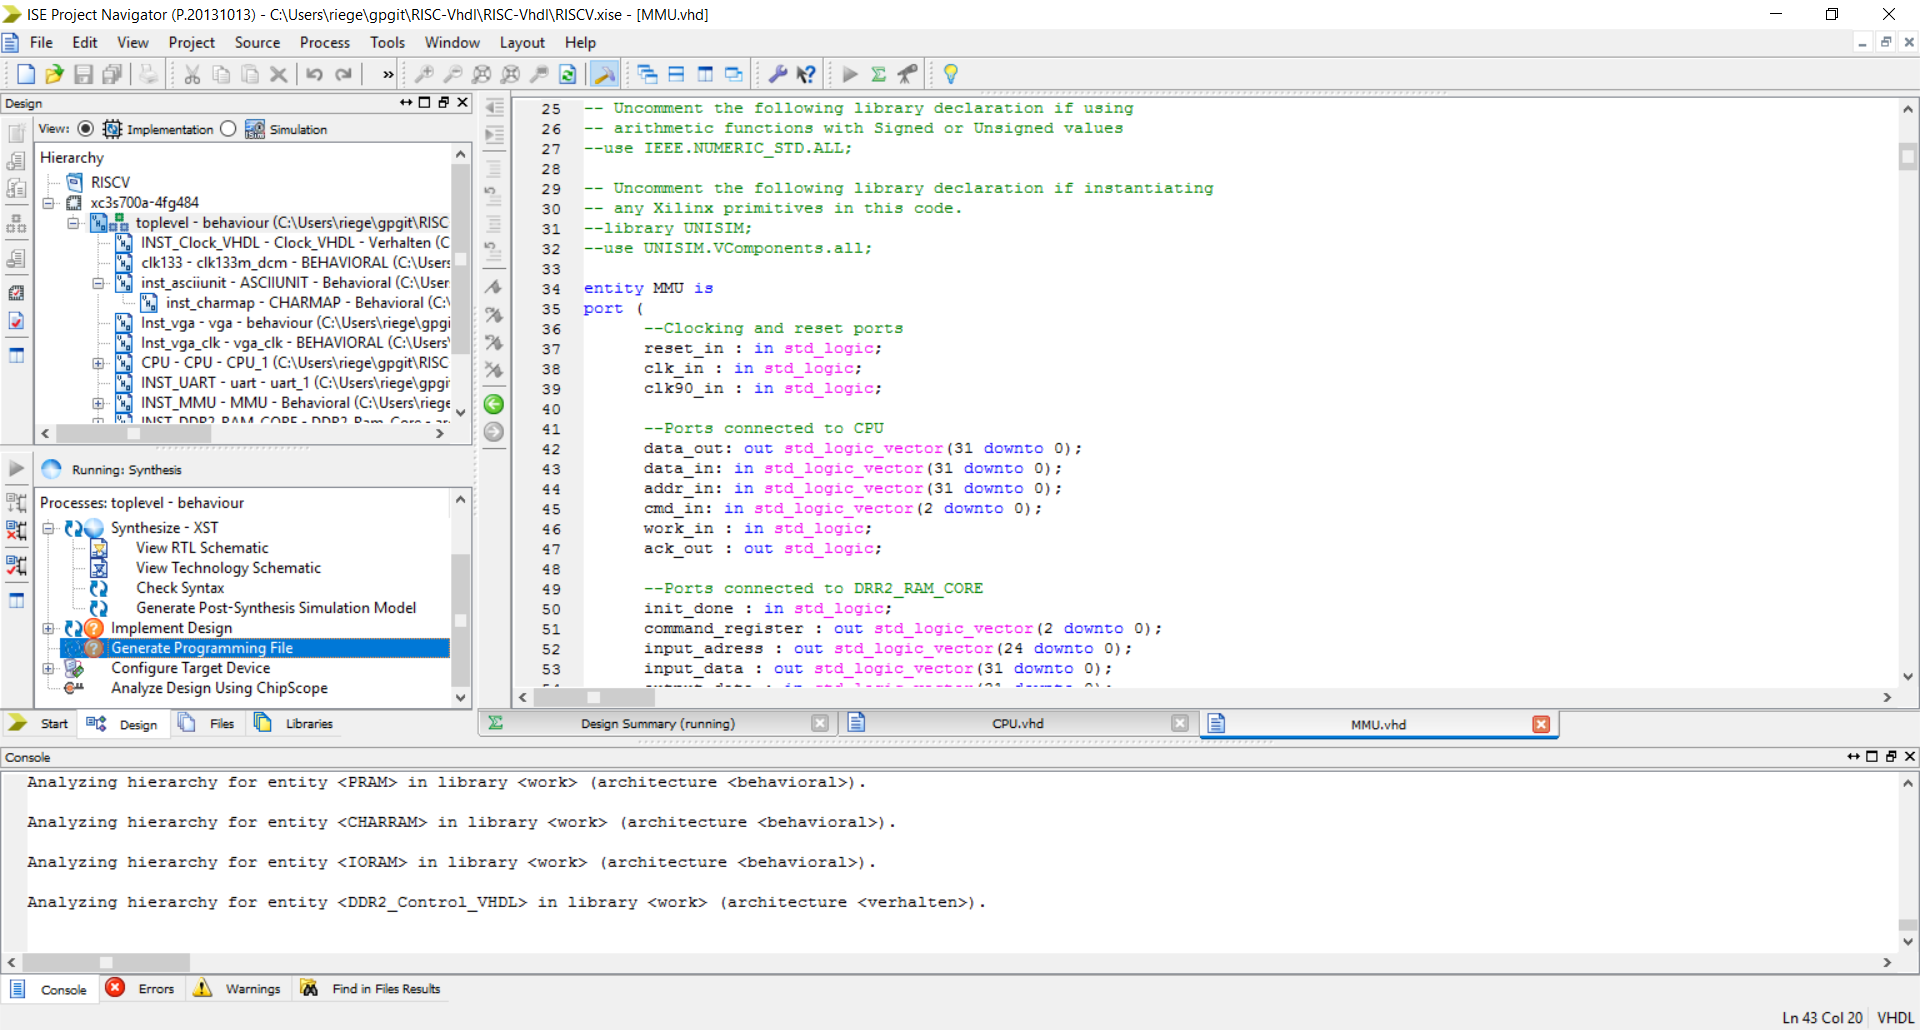
\includegraphics[width=1.0\textwidth]{ISE.png}
	\caption{Der Xilinx ISE Project Navigator}
	\label{fig:tool}
\end{figure}
Mittels Xilinx' \textit{impact} in Kombination mit dem \textit{Cable-Server} wurde das Board dann \"uber USB gem\"a{\ss} den Programming-Files beschrieben.\\
Zur Versionsverwaltung wurde dabei auf ein \textit{Github Repository} gesetzt.\\ 
Um nicht jedes zu testende Programm per Hand assemblieren zu m\"ussen wurde ein Assemblierer auf Python-Basis erstellt.\\
Da die Generierung eines Programming-Files mit anschlie{\ss}endem Beschreiben des FPGAs selbst dann noch jedes Mal mehrere Minuten in Anspruch nimmt, wurden zum schnelleren Testen Simulatoren verwendet. Um den VHDL-Code zu verifizieren wurde so \textit{GHDL} in Kombination mit \textit{GTKWave} verwendet. Auch zur Assemblerprogrammierung wurde ein Simulator mitsamt Textausgabe entwickelt um schneller debuggen zu k\"onnen.
